% document's head

\begin{center}
    \LARGE \textsc{Лабораторная работа № 6.11.2} \\
    \vspace{3 mm}
    \large Исследование фотопроводимости полупроводников
\end{center}

% \hrule

\phantom{42}

\begin{flushright}
    \begin{tabular}{rr}
    % written by:
        % \textbf{Источник}: 
        % & \href{__ссылка__}{__название__} \\
        % & \\
        % \textbf{Лектор}: 
        % & _ФИО_ \\
        % & \\
        \textbf{Автор работы}: 
        & Хоружий Кирилл \\
        & \\
    % date:
        \textbf{От}: &
        \textit{\today}\\
    \end{tabular}
\end{flushright}

\thispagestyle{empty}

\vspace{10mm}


\subsection*{Цель работы}
\begin{enumerate*}
    \item Исследовать собственную фотопроводимость полупроводника.
    \item Определить ширину запрещенной зоны полупроводника из полученной спектральной зависимости.

\end{enumerate*}


\vfill

\begin{figure}[h]
    \centering
    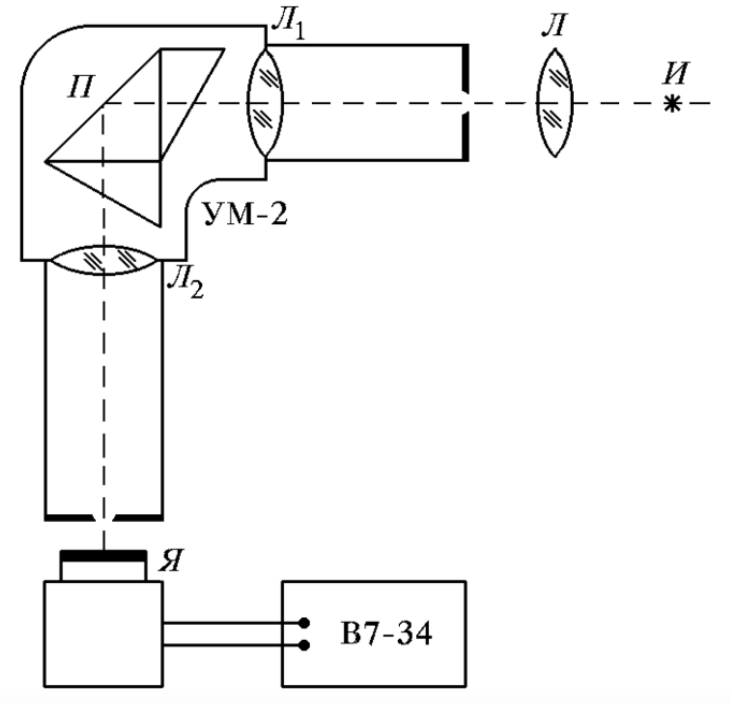
\includegraphics[width=0.35\textwidth]{exp.png}
    \caption{Схема установки}
    \label{fig:exp}
\end{figure}


\subsection*{Оборудование}

\begin{itemize*}
    \item источника И;
    \item монохроматора УМ-2 
    \item линза Л;
    \item вольтметр В7-34.
\end{itemize*}




